\subsection{Galerkin discretisation}
If we take $V_h \subset V$ a finite-dimensional subspace, and consider the discrete problem
\begin{equation}
    \tag{E$_h$}
    \label{eq:Galerkin elliptic variational discrete}
    \text{Find }u_h \in V_h \text{ such that } a(u_h,v_h) = l (v_h) , \qquad \forall v_h \in V_h.
\end{equation}
Since $V_h$ is finite-dimensional, it is also a Hilbert space. And we can apply \namedCref{thm:Lax-Milgram} to show there exists a unique $u_h \in V_h$. The aim of the following sections is to present suitable sub-spaces $V_h$ and estimate $\|u - u_h\|$ is different norms.

\begin{example}[Piece-wise linear functions in $d=1$]
    \label{ex:piece-wise linear in d=1}
    Let us consider the mesh $\{x_0 = 0, x_1, \cdots, x_{N} = 1\}$,
    let $h_i = x_i - x_{i-1}$, and define the mesh parameter $h = \max_i h_i$.
    Formally let $x_{-1}= -\infty$ and $x_{N+1} = +\infty$.
    For such a subdivision, we consider the finite element basis function

    \begin{minipage}{0.95\textwidth}
        \begin{minipage}{0.6\textwidth}
            \[
                \varphi_i(x) \defeq
                \begin{cases}
                    0                            & \text{if } x \leq x_{i-1},       \\
                    \dfrac{x - x_{i-1}}{h_i}     & \text{if } x_{i-1} < x \leq x_i, \\
                    \dfrac{x_{i+1} - x}{h_{i+1}} & \text{if } x_i < x \leq x_{i+1}, \\
                    0                            & \text{if } x_{i+1} < x.
                \end{cases}
            \]
        \end{minipage}
        \begin{minipage}{0.35\textwidth}
            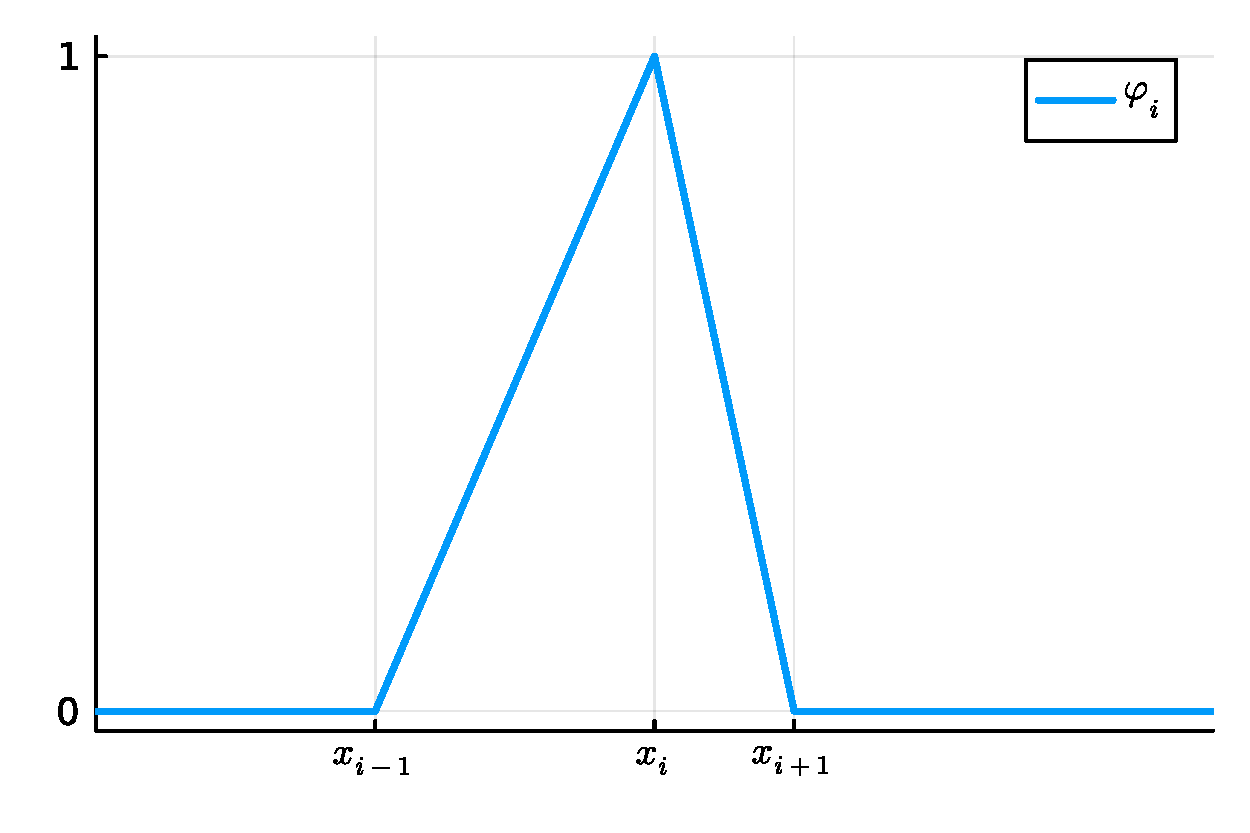
\includegraphics[width=\textwidth]{figures/basis-function}
        \end{minipage}
    \end{minipage}
    If $V = H^1(\Omega)$ (e.g., \Cref{ex:Galerkin Hemholz d=1}) we can take
    \begin{equation*}
        V_h \defeq \spannedby\{\varphi_0, \cdots, \varphi_{N}\}.
    \end{equation*}
    If $V = H^1_0 (\Omega)$ (e.g., \Cref{ex:Galerkin Laplace d=1}) we can take
    \begin{equation*}
        V_h \defeq \spannedby\{\varphi_1, \cdots, \varphi_{N-1}\}.
    \end{equation*}
\end{example}

\begin{example}[Polynomials]
    We can also take $h = N^{-1}$ and $V_h = \mathbb R_N[x]$.
\end{example}
For \namedCref{ex:Galerkin Laplace d=1} we have to take $V_N = \mathbb R_N[x] \cap H_0^1 (\Omega)$. We will discuss suitable basis for this space in the chapter of orthogonal polynomials.

\subsection{Linear Algebra Formulation}
\label{sec:Galerkin elliptic linear algebra}
Suppose that we have the problem $A u = f$ written in weak form as \eqref{eq:Galerkin elliptic variational}.
The finite-dimensional space $V_h$ admits some basis.
Let us drop the $h$ for the remainder of this section and denote a basis of $V_h$ by
\begin{equation*}
    \varphi_1, \cdots, \varphi_{N}
\end{equation*}
We can write
\begin{equation*}
    u_h = \sum_{j=1}^{N} U_j \varphi_j
\end{equation*}
with $U_i \in \mathbb R$.
For \eqref{eq:Galerkin elliptic variational discrete} to hold, it suffices that it holds for every element of the basis.
Taking $v_h = \varphi_i$ in \eqref{eq:Galerkin elliptic variational} we recover
\begin{equation*}
    \sum_{j=1}^{N_h} U_j a(\varphi_j, \varphi_i) = \ell(\varphi_i).
\end{equation*}
Hence, we arrive at the system
\begin{equation}
    \label{eq:Galerkin elliptic linear algebra}
    \mat K \vec u = \vec b, \qquad
    \text{where } \mat K = \Big( a(\varphi_j, \varphi_i)\Big)_{ij},
    \vec u = \left(U_i\right)_i,
    \vec b = \left(\ell(\varphi_i)\right)_i.
\end{equation}
Matrix $\mat K$ is known as the \emph{stiffness matrix} of the operator.
Notice that if $a$ is coercive then $\mat K$ is positive-definite and hence invertible.

\begin{example}[Laplace's equation in $(0,1)$ with piece-wise linear functions]
    We take $N \in \mathbb N$ and $x_0 = 0, x_1 = h, \cdots, x_N = hN = 1$.
    Notice that the basis function $\varphi_0, \varphi_N \notin H_0^1 (0,1)$. We have that
    \begin{equation*}
        a(\varphi_j, \varphi_i) = \int_0^1 \frac{d\varphi_j}{dx} \frac{d \varphi_i}{dx} = \begin{dcases}
            2 / h & \text{if } i = j          \\
            1 / h & \text{if } i = j \pm 1    \\
            0     & \text{if } |i - j| \ge 2.
        \end{dcases}
    \end{equation*}
    Thus, we recover the finite-difference matrix (except the order in $h$)
    \begin{equation*}
        \mat K = \frac 1 {h} \begin{pmatrix}
            2  & -1 &        &        \\
            -1 & 2  & -1              \\

               & -1 & 2      &        \\
               &
               &    & \ddots          \\
               &    &        & -1 & 2
        \end{pmatrix}
    \end{equation*}
    The correct quadratic order in $h$ is still present since
    \begin{equation*}
        b_i = \int_0^1 f \varphi_i \approx h f(x_i)
    \end{equation*}
\end{example}

\subsection*{Exercises}

\begin{exercises}
\item Solve the Galerkin discretisation \namedCref{ex:Galerkin Hemholz d=1} using $V_h = \mathbb R_N[x]$.
When we take as basis $\varphi_k (x) = x^{k-1}$ with $k = 1, \cdots, N-1$ and we have that
\begin{align*}
    K_{ij} & = a(\varphi_j, \varphi_i) = (j-1)(i-1) \int_0^1 x^{j-2} x^{i-2} + \int_0^1 x^{j-1} x^{i-1} dx
    \\
           & = \frac{(j-1)(i-1)}{i+j-3} - \frac{1}{i+j-1}
    \\
    b_i    & = \int_0^1 f(x) x^{i-1} dx.
\end{align*}
Notice that, in this case, $\mat K$ is a full matrix.
It is also interesting to notice that, unlike with finite-difference methods, the approximate solution $u_h$ does not in general satisfy the Neumann boundary conditions.
\end{exercises}